% Copyright (c) 2017 Ongun Kanat <ongun.kanat@gmail.com>
% Permission is hereby granted, free of charge, to any person obtaining a copy of 
% this software and associated documentation files (the "Software"), to deal in 
% the Software without restriction, including without limitation the rights to 
% use, copy, modify, merge, publish, distribute, sublicense, and/or sell copies of 
% the Software, and to permit persons to whom the Software is furnished to do so, 
% subject to the following conditions:
% 
% The above copyright notice and this permission notice shall be included in all 
% copies or substantial portions of the Software.
% 
% THE SOFTWARE IS PROVIDED "AS IS", WITHOUT WARRANTY OF ANY KIND, EXPRESS OR 
% IMPLIED, INCLUDING BUT NOT LIMITED TO THE WARRANTIES OF MERCHANTABILITY, FITNESS 
% FOR A PARTICULAR PURPOSE AND NONINFRINGEMENT. IN NO EVENT SHALL THE AUTHORS OR 
% COPYRIGHT HOLDERS BE LIABLE FOR ANY CLAIM, DAMAGES OR OTHER LIABILITY, WHETHER 
% IN AN ACTION OF CONTRACT, TORT OR OTHERWISE, ARISING FROM, OUT OF OR IN 
% CONNECTION WITH THE SOFTWARE OR THE USE OR OTHER DEALINGS IN THE SOFTWARE.

% Copyleft (ɔ) 2018 Mehmet Tahir SANDIKKAYA <sandikkaya@itu.edu.tr>
% Corrected( and especially prepared for my own students).
% I added my initials as in here where I corrected. -MTS

% 12pt and ISO A4 paper
\documentclass[a4paper, 12pt]{article}

% I added a bit more options for better organization. -MTS
\newif\ifturkish
\newif\ifdraft
\newif\ifcover

% Toggle the following options by commenting them in or out for possible rendering options. -MTS

%\turkishtrue
%\drafttrue
\covertrue


% Margins and page size
\usepackage[a4paper,top=2.5cm,bottom=2.5cm,left=3.3cm,right=2.2cm]{geometry}

% Page headers are set to top right
\usepackage{fancyhdr}
\pagestyle{fancy}
\renewcommand{\footrulewidth}{0pt} % clear rulers
\renewcommand{\headrulewidth}{0pt}
\lhead{} % Empty left header
\rhead{\thepage} % Page number at the right header
\cfoot{} % Clear center of the footer
% To get rid of annoying warning message... -MTS
% Does not really affect formatting.
\setlength{\headheight}{15pt}

% NOOOO! Commenting out! -MTS
% Use American English for dates etc.
%\usepackage[american]{babel}
% If document is in Turkish then use
% \usepackage[turkish]{babel}
% or for both
% \usepackage[turkish,american]{babel}

% Indent at section beginnings
%\usepackage{indentfirst}
% Do NOT uncomment this if it is not specifically asked for. -MTS
% The original template requires the first paragraph to be unindented. -MTS

% utf-8 support

% No no no! -MTS
% First, you should load the font.
% Then, add UTF-8 support. Otherwise, the font cannot display UTF-8.
% Oh, man!
\usepackage[T1]{fontenc}
\usepackage[utf8]{inputenc}
%\usepackage[turkish,english]{babel}
%\usepackage[english,turkish]{babel}
% Then, you can start hyphenation and language support.
% Please, follow the logical order. -MTS

\ifturkish
	\usepackage[english,turkish]{babel}
\else
	\usepackage[turkish,english]{babel}
\fi

% <MTS>
% Şimdi işin çetrefilli bölümüne geliyorum.
% Bu kısım Türkçe yazanları ilgilendiriyor.
% Ancak, İngilizce yazanlar da hiç değilse Özet'i Türkçe yazarken
% heceleme kullanmak isteyebilirler.
% babel paketi hecelemeye yardım eder.
% Ancak babel Türkçe desteği verirken 
% son 666 yıldır graphicx paketi ile çakışır.
% Bu nedenle \includegraphics içinde '=' kullanamazsınız.
% Ne yapılabilir?
% Evet, graphicx kullanmadan önce '=' kullanımına anlam yitirtirsiniz.
% Sonra anlamını geri verirsiniz. Örnek kullanım şöyle:

%    \shorthandoff{=}
%    \includegraphics[width=\linewidth]{gantt_diagram.png}
%    \shorthandon{=}

% Önemli bir not daha: babel'a hangi dili son sırada yazarsanız
% adını belirtemediğiniz toc, lot, lof gibi başlıklarınızın dili
% o dilde görünür.
% O nedenle Türkçe tez yazıyorsanız babel oarametrelerinin sırasını değiştirin.
% Ki, içindekiler, tablo listesi, vb. Türkçe başlıklarınız olsun.
% </MTS>

% Graphics for PDFTeX
\usepackage[pdftex]{graphicx}
% Lütfen vektör grafikler kullanın.
% jpg, png kullanmayın.
% Derleme sırasında pdftex derleyicisi kullanıyorsanız (ki varsayılan bu)
% zaten pdf formatında hazırladığınız figürler vektör formatında kalite
% kaybı olmadan görünür. -MTS

% Figure placement
\usepackage{float}

% An enumeration package for flexible enumeration
\usepackage{enumitem}

% For fitting tables into the page width
\usepackage{makecell}
\renewcommand{\theadalign}{cc} % Centering and at the middle
\renewcommand{\theadfont}{\bfseries} % Bold table headers

% Helvetica Sans-serif fonts
\usepackage{helvet}
\usepackage{sectsty}
\allsectionsfont{\normalfont\sffamily\bfseries}
\sectionfont{\fontsize{18pt}{21.6pt}\sffamily\bfseries}
\subsectionfont{\fontsize{16pt}{19.2pt}\sffamily\bfseries}
\subsubsectionfont{\fontsize{14pt}{16.8pt}\sffamily\bfseries}

% Courier monospace font
\usepackage{courier}

% Table of contents dot fill, sans serif header and name change
\usepackage{tocloft}
\renewcommand{\cftsecleader}{\cftdotfill{\cftdotsep}}
\tocloftpagestyle{fancy}
\renewcommand{\cfttoctitlefont}{\sffamily\Large\bfseries}
\setlength{\cftbeforesecskip}{6pt}
\renewcommand{\contentsname}{Table of Contents}

% Links, both local and external
\usepackage{hyperref}
\hypersetup{
	unicode=true,
	colorlinks=true,
	urlcolor=blue,
	citecolor=black,
	menucolor=black,
	linkcolor=black
}
% colorlinks parametresini false yapın ki linkler mavi mavi sırıtmasın. -MTS

% Figure captions are bold
\usepackage[labelfont=bf,font=sf]{caption}

% Pseudocode from algorithmicx package
\usepackage{algorithmicx}
\usepackage{algpseudocode}
\usepackage[section,boxed]{algorithm}
\captionsetup[algorithm]{labelfont=bf,font=sf,justification=centering,position=top}

% Listings for implemented code
\usepackage{listings}
\lstset{basicstyle=\ttfamily,frame=lines,tabsize=4}
\renewcommand{\lstlistingname}{Listing}

% A powerful math notation package
\usepackage{amsmath}

% To set lowercase/uppercase. -MTS
% Helpful for automating cover page. -MTS
\usepackage{textcase}

% To generate pretty looking tables. -MTS
% Please stick with it. -MTS
\usepackage{booktabs}

% A packege for graphics. -MTS
% You just need to include data here. It will draw. -MTS
\usepackage{pgfplots}
\pgfplotsset{compat=1.14}
% You may add extra libraries, if required. -MTS
\usepgfplotslibrary{polar}

% <MTS>
% The package for assigning linenumbers with the command \linenumbers
% Helpful during the draft phase to point out any specific place in the manuscript.
% Must be commented out before submitting the thesis.
% </MTS>
\ifdraft
	\usepackage{lineno}
	\linenumbers
\else
\fi

% <MTS>
% ALWAYS set all fields. Both title and baslik in both languages.
% They will be visible in the cover and summary pages.
% Title, author and date info variables for later use.
% </MTS>
\title{Name of the Graduation Project}
\author{Merve CANDAN}
\date{October 2020}
\def\baslik{Bitirme Procesinin Adı ve Sanı}
\def\BASLIK{BİTİRME PROCESİNİN ADI VE SANI}% BÜyük harf ile yazımda i, I'ya dönüştüğü için...
\def\studentId{150160041}
\def\faculty{Faculty of Computer And Informatics}
\def\fakulte{Bilgisayar ve Bilişim Fakültesi}
\def\department{Computer Engineering}
\def\division{Computer Engineering}
\def\bolum{Bilgisayar Mühendisliği}
\def\program{Bilgisayar Mühendisliği}
\def\advisor{Asst. Prof. Dr. Mehmet Tahir SANDIKKAYA}
\def\danisman{Yard. Doç. Dr. Mehmet Tahir SANDIKKAYA}
\def\tarih{Haziran 2018}% Ay/Yıl olarak tarih yazılırken Türkçeleşmediği için.
\def\signPlace{İstanbul}
\def\signDate{\today}

\ifturkish%
	\def\ozbil{%
\section*{Özgünlük Bildirisi}
\begin{enumerate}
    \item Bu çalışmada, başka kaynaklardan yapılan tüm alıntıların, ilgili kaynaklar referans gösterilerek açıkça belirtildiğini,
    \item Alıntılar dışındaki bölümlerin, özellikle projenin ana konusunu oluşturan teorik çalışmaların ve yazılım/donanımın tarafımdan yapıldığını
    bildiririm.
\end{enumerate}
\vspace{1em}
\signPlace, \signDate
\vspace{3em}\\
}%
\def\ack{Teşekkürler}%
\else%
	\def\ozbil{%
\section*{Statement of Authenticity}
I hereby declare that in this study
\begin{enumerate}
    \item all the content influenced from external references are cited clearly and in detail,
    \item and all the remaining sections, especially the theoretical studies and implemented
software that constitute the fundamental essence of this study is originated by my individual authenticity.
\end{enumerate}
\vspace{1em}
\signPlace, \signDate
\vspace{3em}\\
}%
\def\ack{Acknowledgements}%
\fi%

% Bozuk heceleme olursa burada düzeltin.
\hyphenation{boş-luk ve-re-rek is-te-di-ği-miz ka-dar söz-cük ya-za-bi-li-riz in ev-ery lan-guage to-geth-er}


\begin{document}
\numberwithin{figure}{section}
\numberwithin{table}{section}
\numberwithin{lstlisting}{section}

\ifcover

\makeatletter
\ifturkish
	\begin{titlepage}
    \bfseries % Make all text bold in this environment
    \sffamily % Similarly select sans-serif font
	\begin{center}
		\LARGE{\textbf{İSTANBUL TEKNİK ÜNİVERSİTESİ\\ 
               \MakeTextUppercase{\fakulte}} } \\
		\vspace{5.5cm}
		\LARGE{\MakeTextUppercase{\BASLIK}}\\
		\vspace{4.5cm}
		\Large{Bitirme Projesi} \\
        \vspace{0.5cm}
		\Large{\@author} \\
     	\Large{\studentId} \\
        \vspace{4cm}
        \large{Bölüm: \bolum} \\
        \large{Program: \program} \\
        \vspace{1.5cm}
        \large{Danışman: \danisman} \\
		\vspace{\fill} % Fill out until the page end
		\large{\normalfont \sffamily \tarih}
	\end{center}
	\end{titlepage}
\else
	\begin{titlepage}
    \bfseries % Make all text bold in this environment
    \sffamily % Similarly select sans-serif font
	\begin{center}
		\LARGE{\textbf{ISTANBUL TECHNICAL UNIVERSITY \\ 
               \MakeTextUppercase{\faculty}} } \\
		\vspace{5.5cm}
		\LARGE{\MakeTextUppercase{\@title}}\\
		\vspace{4.5cm}
		\Large{Graduation Project} \\
        \vspace{0.5cm}
		\Large{\@author} \\
     	\Large{\studentId} \\
        \vspace{4cm}
        \large{Department: \department} \\
        \large{Division: \division} \\
        \vspace{1.5cm}
        \large{Advisor: \advisor} \\
		\vspace{\fill} % Fill out until the page end
		\large{\normalfont \sffamily \@date}
	\end{center}
	\end{titlepage}
\fi

\pagenumbering{Roman} % Capital roman numerals as page numbers
\newpage
\ozbil\@author\newpage
\section*{\ack}
If you do not want to acknowledge anyone, delete the whole section. Otherwise, thank Knuth designing \TeX .

\newpage
\section*{\@title}
\centerline{\large\bfseries (Summary)}

\par Attackers constantly try to hack all devices that are connected to the internet by exploiting various vulnerabilities. During that process they do not filter any devices and try to attack every device that they can reach. To analyze and notice such attacks there is concept which is called honeypots. Honeypots act like a normal device but they are special devices and the attackers send their viruses to these devices as well. 

\par In this project, the aim is to automate the analyzing process. We will emulate various kinds of devices using Raspberry Pi computers. We will buy VPC services all around the world and stream all incoming data by using UDP protocol to our Raspberry Pi's. Our devices will be managed using a master device and attacks will be analyzed on that device.

\newpage
\section*{\baslik}
\centerline{\large\bfseries (Özet)}
Türkçe tezler için kısa özet yazınız. 1 ya da 2 sayfa. İngilizce tezler için geniş özet yazınız. 2 ya da 3 sayfa.

\newpage
\tableofcontents
\newpage
\listoffigures
\newpage
\listoftables
\newpage
\makeatother

\else
\fi

% For the ones who doesn't know: 1,2,..9 called West Arabic numbers
\pagenumbering{arabic}
\section{Introduction}
%Raporlanmanın hızlanması, şu anda bir sürü saldırı yapılıyor, güvenliğin artmasına yardımcı olacak. Daha hızlı ve daha güvenli bir sistem oluşacak. Honeypotların yaygınlaşmasını sağlayacak. Bilinmeyen ya da yeni üretilen virüs türlerini bulabileceğiz, başka firmaların analiz için bizim sistemimizi kullanmasını bekliyoruz. Virüs türlerinin yüzdeleri, ne sıklıkla saldırdığı.%
With the advancing technology, many cyber attacks are taking place these days in various ways. Devices that contain the Internet of Things technology are becoming more common. As a result, different security vulnerabilities occur in this new industry. IoT is the connection between devices connected to the common network and between the user and the device. A lot of technological devices can be given as examples of IoT devices. For example, smart home systems, cameras, phones etc. This technology continues to evolve, and as it continues, new types of viruses or new types of attacks may emerge. In the intended project, we aim to accelerate the reporting of these attacks, increase security, create a faster system, and detect unknown or newly produced virus types by using the system to be established. In doing so, we will set up servers called Honeypot that acts like other devices, and we will set traps where we can get information about where and how the attack happened when an attack occurs. We plan to achieve a worldwide result by placing these Honeypot servers in multiple continents and various countries. Attacks on honeypot servers will be reported simultaneously using real-time system software.

\newpage
\section{Project Description and Plan}
This is the best graduation project ever. In Figure \ref{fig:ganttdiagram} you can see the Gantt diagram of the project.
Pert chart çizilcek, 1-araştırma,1.1- linux bash ve network mimarisi öğrenme,  2- başka honeypot sistemleri incelenecek, 3-sistem kurulmaya başlancak, 4- ara rapor, 5-internet sitesinin hazırlanması, 6- sistemin online olması, 7-rapor

\begin{figure}[H]
    \centering
    \shorthandoff{=}
    \includegraphics[width=\linewidth]{gantt_diagram.png}
    \shorthandon{=}
    \caption{The Gantt diagram of the project, which is not good. Try to come up with parallel tasks in time. So that, if you fail at any step, rest of the steps are not (or less) affected.}
    \label{fig:ganttdiagram}
\end{figure}

\newpage
\section{Background}
A long long section with many papers. Include previous related work. A short history (I said short). Compare and relate all other works with yours.
%Diğer honeypotlardan farkı yazılacak, bizimki otomatik analiz yapabilecek. Bütün teknik detaylar. Bu konu hakkında diğer çalışmalar%
Honeypot is a computer system used to attract cyber attacks as a bait for computer security. It imitates a device and uses attack attempts to obtain information or distract criminals and their way of working from other targets. It was usually done manually to examine the virus detected in systems installed until now. We aim to automatically analyze the Honeypot servers we will establish.

\newpage
\section{Analysis and Modeling}
After long hours of studying we decided. A* is the best algorithm for searching on the graphs.

Bulunan yollardan hangisi best fit, neden o? Modellemesi nasıl

\newpage
\section{Design and Implementation}
We implemented the depth first search algorithm as shown in Algorithm

sistemin şekli çizilecek, sistem detaylı anlatılacak.

\ref{algo:dfs}.
\begin{algorithm}[H]
    \caption{The depth first search algorithm}
    \label{algo:dfs}
    \begin{algorithmic}[1]
        \State \textbf{Graph} $G$
        \State \textbf{Node} $start$
        \Function{Depth-First-Search}{$G$, $start$}
        \State \textbf{Tree} $ T $ \Comment The resulting search tree
        \State \textbf{Stack} $ S $ \Comment An empty stack
        \State \textbf{Set} $ V $ \Comment An empty set of visited nodes
        \State \Call{set-root}{$ T $,$ current $}
        \State \Call{push}{$ S $,$ start $}
        \While{\Call{not-empty}{S}}
        \State $current \gets$ \Call{pop}{$ S $}
        \If{\textbf{not} \Call{Contains}{$ V $, $ current $} }
        \State \Call{insert}{$ V $, $ current $}
        \ForAll{$ n $ : \Call{neighbors}{$ current $} }
        \State \Call{push}{$ S $, $ n $}
        \State \Call{insert-sub-node}{$ T $, $ current $, $ n $}
        \Comment Insert node to subtree of $ current $
        \EndFor
        \EndIf
        \EndWhile
        \State \Return $ T $
        \EndFunction
    \end{algorithmic}
\end{algorithm}

\newpage
\section{Testing and Evaluation}
We compared the performance of the graph search algorithms. The results can be seen in the Table

Elde ettiğimiz veriler. Virüslerin yüzde kaçı eski,yeni
\ref{tbl:results}.

\begin{table}[H]
    \caption{Performance test results of the graph search algorithms}
    \label{tbl:results}
    \centering
    \begin{tabular}{|c|r|r|r|} 
        \hline 
        \thead{Algorithm} & \thead{Number of \\ Generated Nodes} & \thead{Number of \\ Nodes Expanded} & \thead{Max Number of \\ Nodes in The Frontier} \\ 
        \hline 
        BFS &  77480 & 6340 & 71142 \\ 
        \hline 
        DFS & 820 & 88 & 760 \\ 
        \hline 
        A* & 376 & 33 & 338 \\ 
        \hline 
    \end{tabular}
\end{table}

\begin{table}[H]
    \centering
    \caption{It is always better to use booktabs package for tables. Then, you can generate pretty looking tables. Advise: never use vertical lines in your tables. Rule: captions are below figures and above tables.}
    \begin{tabular}{rcl}
        \toprule
         Header & Header & Header \\
         \midrule
         Value & Value & Value \\
         \bottomrule
    \end{tabular}
    \label{tab:my_label}
\end{table}

\begin{figure}[H]
\begin{tikzpicture}
  \begin{axis}
    \addplot+[sharp plot] coordinates
      {(0,0) (1,2) (2,3)};
  \end{axis}
\end{tikzpicture}
\caption{Isn't it nice to use some graphs?}
\end{figure}

\begin{figure}[H]
\centering
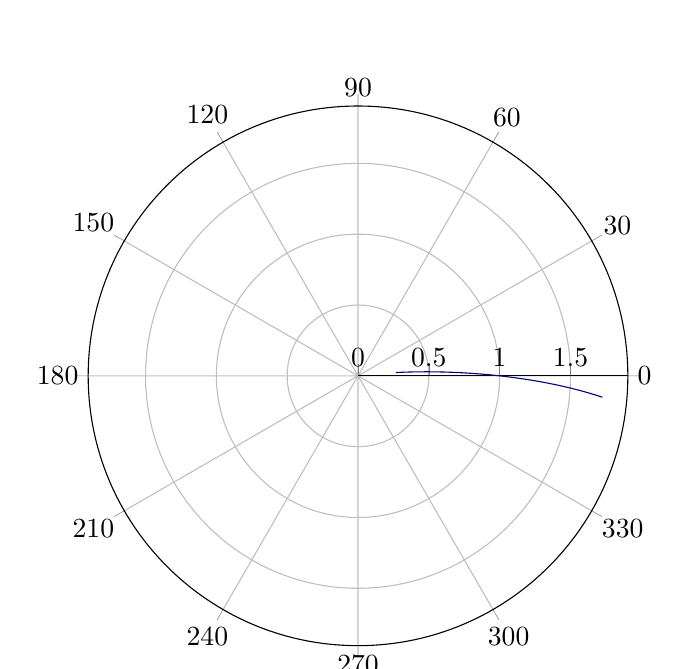
\begin{tikzpicture}
  \begin{polaraxis}[
      domain = -3600:3600,
      samples = 4000
    ]
    \addplot[blue!50!black] {1 - sin(50*x/49) - sin(8*x)};
  \end{polaraxis}
\end{tikzpicture}
\caption{Or, maybe a flower}
\end{figure}

\newpage
\section{Conclusion and Discussion}
We tested algorithms and decided that future is bright.

\newpage
\bibliographystyle{IEEEtran}
\bibliography{references.bib}

\end{document}
